\section{Interface Data Structures}\label{interface-data-structures}

We will refer to several data structures throughout the discussion of
user interface design and implementation. These are the primary means of
storing user input processed by the tools, and are processed by our
algorithms to draw designs in 2D and simulate them 3D\footnote{This
  section only describes the primary data structures necessary for
  constructing fold and patterns from user input, detecting planes, and
  determining the relationships between, not the systems for drawing
  features in 2D or 3D. For a discussion of 2D drawing, see sections.
  For a discussion of, see .
  \textbf{\textgreater{}\textgreater{}TODO:cite marissa
  \textgreater{}\textgreater{}TODO reference section}}.

\subsection{Edges}\label{edges}

An Edge represents a cut or fold. Edges are the basic building block of
planes, and an integral element of all fold features. An edge is
minimally defined by a start point, end point, and a a type (either cut
or fold). This minimal definition represents a straight edge between two
points. In addition, an Edge can contain further information: the bezier
path drawn to create it (for non-straight edges), and a reference to the
plane or feature it is a part of. Additionally, each edge contains a
reference to its ``twin'' edge.

\subsubsection{Twin Edges}\label{twin-edges}

Although it is often simplest to think of edges as cuts and folds
created by the user, the reality in Foldlings is slightly more
complicated. For each edge that the user creates using a tool, two edges
are created. We create edges with direction, such that there is an edge
from the start point to the end point of the edge, and another edge
starts at the endpoint and has the reverse path of the original edge.
This distinction is most important when detecting planes from
edges\footnote{\textbf{\textgreater{}\textgreater{}TODO cite marissa's
  planes}}, but must also be taken into account whenever edges are
processed. For example, when drawing the 2D view of a sketch, we skip
drawing the twins of edges already drawn, which reduces drawing work by
half.

\begin{figure}[htbp]
\centering
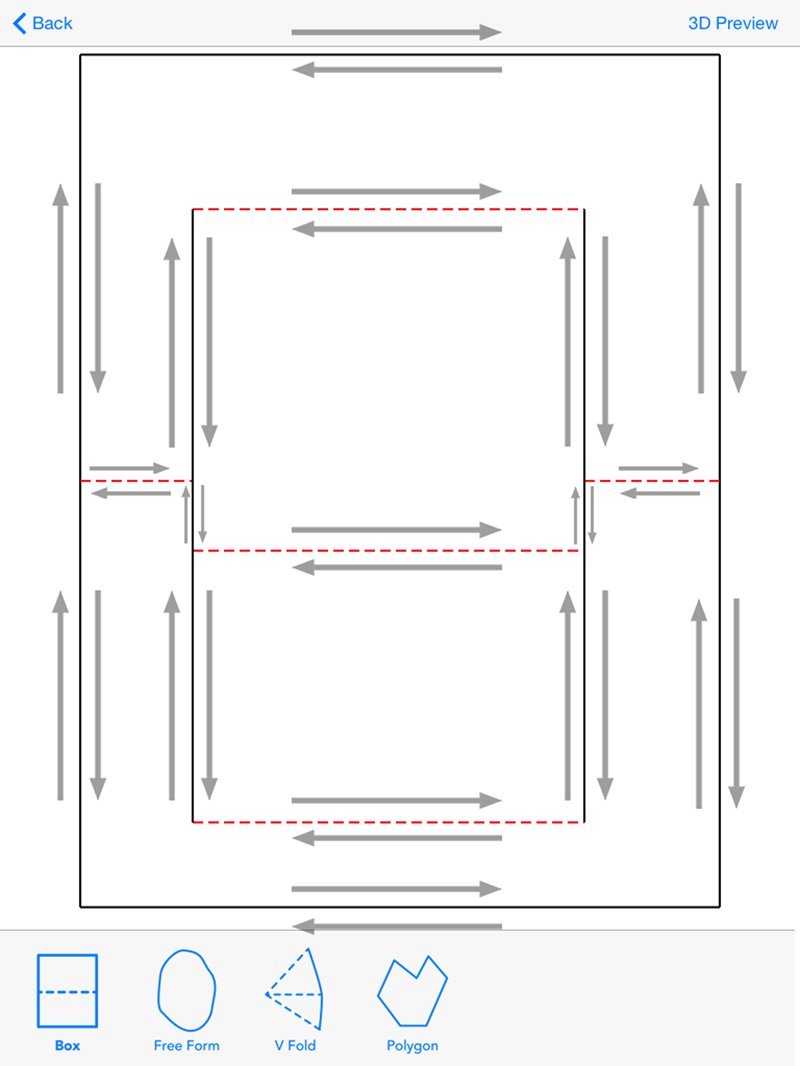
\includegraphics{figures/33_UI_Interface_Data_Structures/boxfold_34_edges.png}
\caption{This sketch contains 34 edges, with orientations shown by the
overlaid gray arrows.}
\end{figure}

\subsubsection{Driving Folds}\label{driving-folds}

A driving fold is not a special type of edge, but rather a relationship
between an edge in one feature and a feature ``spanning'' that edge. A
feature is said to span a fold when it is drawn on top of an existing
fold, so that it has horizontal folds on both sides of the middle fold.

\begin{figure}[htbp]
\centering
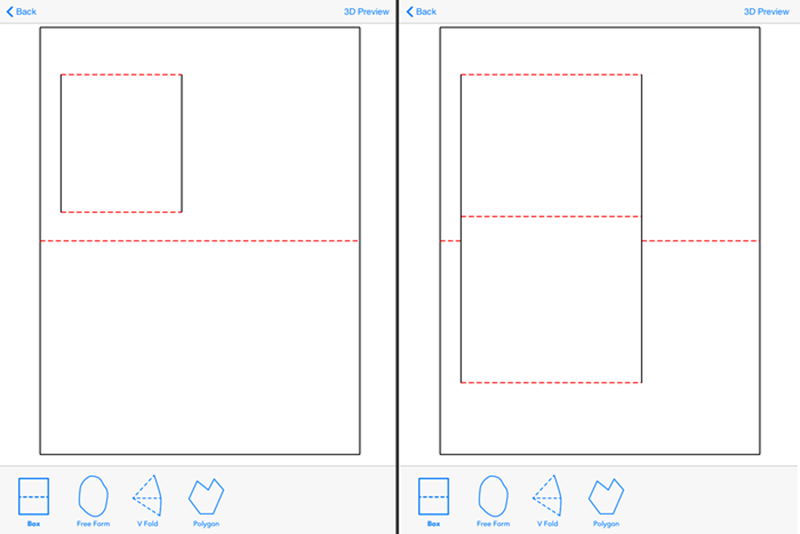
\includegraphics{figures/33_UI_Interface_Data_Structures/boxfold_driving_non_driving.png}
\caption{Left: a box fold mid-drag. The feature does not have a driving
fold. Right: a box-fold after the user has released the touch. The
feature's driving fold is the master card's middle horizontal fold.}
\end{figure}

An edge can be the driving fold for more than one feature, but each
feature has only one driving fold (if there are multiple potential
driving edges at the same height, the leftmost edge is selected. The
driving fold is important for calculating parent-child relationships
between features: a feature's parent is the feature that contains it's
driving fold\footnote{The exception to this rule is holes ---~a hole's
  parent is the feature that contains it.}. These parent-child
relationships are described in more detail in the
\nameref{nested-features} section on page \pageref{nested-features}.

\subsubsection{Fold Orientation}\label{fold-orientation}

Traditionally, kirigami patterns indicate direction for folds:
``mountain/hill'' or ``valley''. These folds form angles in opposite
directions ---~mountain folds are pinched away from the paper surface,
while valley folds are pinched into the surface.
\textbf{\textgreater{}\textgreater{}TODO: FINISH SECTION, CITE KIRIGAMI
HERE, REFERENCE MARISSA} \textbf{\textgreater{}\textgreater{} TODO
KIRIGAMI PATTERN FIGURE}

\subsection{Planes}\label{planes}

Planes are an enclosed shape, bounded by edges. Plane are detected from
edges by traversing the directed edge graph, as described in
\textbf{\textgreater{}\textgreater{}TODO: CITE MARISSA HERE}. They are
drawn as colored areas in the two-dimensional sketch, and simulated in
the 3D preview as shapes that rotate about a pivot point. In order to
simulate the planes in 3D, we construct parent-child relationships
between the planes, which determine how they move during simulation.

\begin{figure}[htbp]
\centering
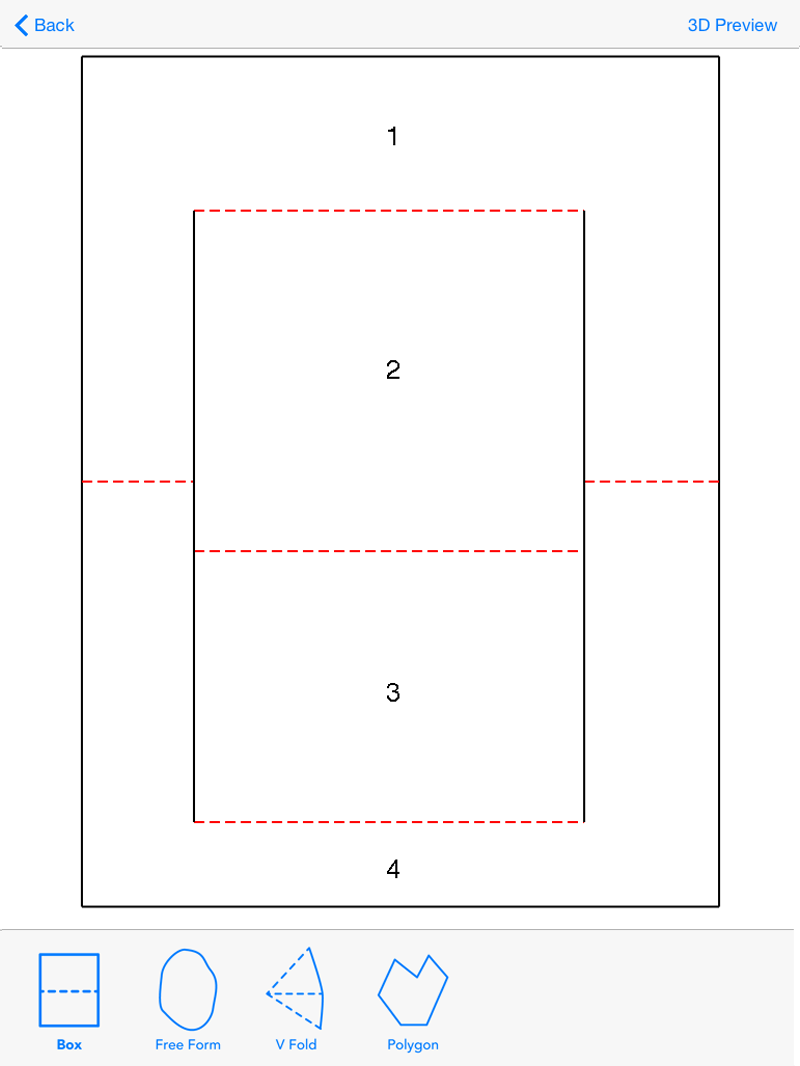
\includegraphics{figures/33_UI_Interface_Data_Structures/boxfold_planes.png}
\caption{Planes in a simple sketch, numbered by ancestry. Starting at
the root plane 1, each successive plane is the child of the previous
numbered plane.}
\end{figure}

\subsection{Fold Features}\label{fold-features}

The central data structure of Foldlings is the FoldFeature: a
representation of a shape drawn by the user that folds in 3d. Each fold
feature is a single design element ---~and can be individually created,
modified, and deleted. There are five classes of FoldFeature:
MasterCard, BoxFold, FreeForm, Polygon, and V-Fold, representing
differences in drawing behavior, geometry, and (the differences are
described in detail below). Each of these features is a subclass of the
FoldFeature superclass.

All FoldFeatures have functionality in common:

\begin{itemize}
\itemsep1pt\parskip0pt\parsep0pt
\item
  Each feature contains a list of edges in the feature ---~cuts and
  folds, including twins.
\item
  Each feature has a driving fold --- in the case of unconnected
  features, such as the master card and holes, the driving fold is nil.
\item
  Each feature can be deleted from the Sketch, ``healing'' the sketch by
  closing gaps left in any
\item
  Features implement the encodeWithCoder and decodeWithCoder methods,
  allowing them to be serialized to a file on the device and restored
  from the saved file.
\item
  Each feature can provide a list of current ``tap options'' --- actions
  that can be performed on the feature given its state.
  \textbf{\textgreater{}\textgreater{}TODO:SEE tap options in interface
  design}
\item
  Each feature can perform hit-testing: given a point, it can determine
  whether that point is inside or outside the feature. \citep{Nobody06}.
  \textbf{\textgreater{}\textgreater{}TODO:REMOVE CITATION -- JUST
  TESTING}
\end{itemize}

\subsubsection{Master Card}\label{master-card}

Each sketch always contains a single master feature, which is the
ancestor of all other features. It is a simplification of the box fold,
in that it contains three horizontal folds with connecting vertical
cuts. Users do not create features of this type~--- each sketch begins
with one. All of the edges in the master feature are marked with a flag
indicating that they belong to the master feature, because master
feature edges and planes are sometimes treated differently than normal
edges. For example, the parent-child relationships between planes are
constructed by starting at the top plane in the master feature,
determined by edge type and height.

\subsubsection{Box Fold}\label{box-fold}

A box fold consists entirely of straight edges, and can be constructed
from two points: the top left point, and the bottom right. The middle
fold position is determined by the position of the driving fold. Box
folds are only valid if they have a driving fold.

\subsubsection{Free Form}\label{free-form}

Free-form shapes are defined by a single, closed path. When the feature
is completed (by releasing the touch), the shape is truncated,
horizontal folds are added, and the path is split into multiple edges
(assuming the shape spanned a fold)\footnote{\textbf{\textgreater{}\textgreater{}TODO:SEE
  SECTION}}. The curved path is defined by a set of ``interpolation
points'' ---~points captured by sampling touch positions while a user
draws a shape on the screen. A bezier path is interpolated between these
points using the Catmull-Romm algorithm \textbf{TODO: CITE}.

Holes are a special case of FreeForm shapes, and are cut out from the
final design, rather than simulated as a separate plane. FreeForm shapes
that do not cross a fold are considered holes ---~drawn in white in the
2d sketch and drawn as subtractions from planes in the 3d view.

\subsubsection{Polygon}\label{polygon}

Polygons are created from a list of ``tap points'' constructed from user
input. As in free-form shapes, these points are connected with a bezier
path, and are truncated if they contain a driving fold when they are
completed. For polygons, this path consists only of straight line
segments. Unlike interpolation points, tap points can be moved at any
time during the drawing process.

Like FreeForm shapes, Polygons that do not have a driving fold are
considered holes.

\subsubsection{V-Fold}\label{v-fold}

V-Folds are defined by a path that crosses the driving fold, called a
``vertical cut.'' This path can be an arbitrary shape that crosses the
driving fold once. They are fully-defined by adding a point on the
driving fold. From this point, we construct three diagonal folds, two to
the top and bottom of the vertical cut, and one to a point that
intersects with the vertical cut at a point calculated to make a valid
90-degree feature.

\begin{figure}[htbp]
\centering
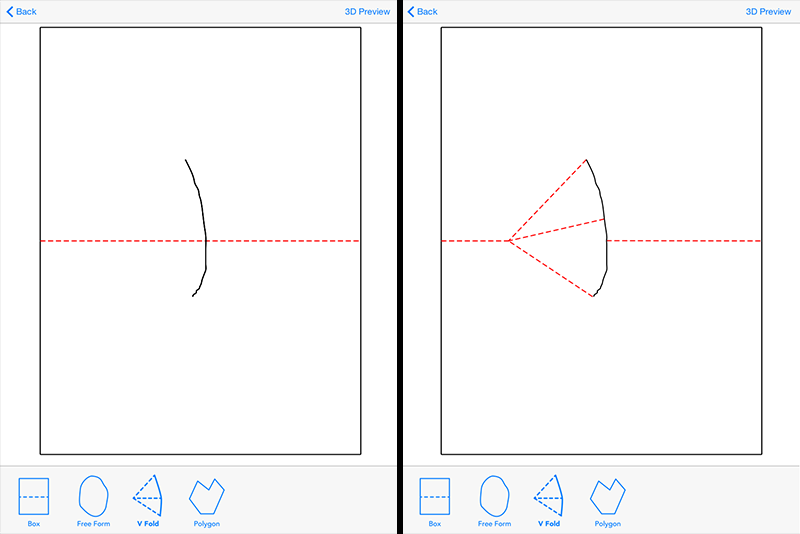
\includegraphics{figures/33_UI_Interface_Data_Structures/vfold_before_after.png}
\caption{Left: an unfinished v-fold, consisting only of a vertical cut.
Right: a v-fold after defining the point on the driving fold to create
diagonal cuts.}
\end{figure}

V-folds are only valid if they have a driving fold, and their vertical
cut intersects the driving fold exactly once.

\subsection{Sketches}\label{sketches}

A sketch is the representation of the user's drawing ---~its primary
role is as a collection of features. It also contains information about
the current drawing state, and the state of user interaction (for
example, which features are currently being modified, and which tool is
selected).
